% dimensions(x) returns number of spatial dimensions
% y = transform(x, "proj4string")
% bbox(x)
% coordinates(x) ; <-
% rings(x) ; <-
% method to retrieve lines? --> Lines()?
% gridded(x)  ; <-
% 
\documentclass{article}

\usepackage{graphicx}
\usepackage[colorlinks=true,urlcolor=blue]{hyperref}

% \VignetteIndexEntry{ sp: overlay and aggregation }

\usepackage{color}

\usepackage{Sweave}
\newcommand{\strong}[1]{{\normalfont\fontseries{b}\selectfont #1}}
\newcommand{\code}[1]{{\tt #1}}
\let\pkg=\strong

\title{\bf Map overlay and \\ spatial aggregation in {\tt sp}}
\author{Edzer Pebesma\footnote{Institute for Geoinformatics,
University of Muenster, Weseler Strasse 253, 48151 M\"{u}nster, Germany.
{\tt edzer.pebesma@uni-muenster.de}}}
\date{\today}

\begin{document}
\Sconcordance{concordance:over.tex:over.Rnw:%
1 103 1 1 2 1 0 1 1 3 0 1 2 7 1 1 2 4 0 2 2 4 0 2 2 1 0 5 1 1 2 1 1 1 7 %
9 0 1 2 2 1 1 13 1 2 4 1 1 2 8 0 1 2 4 1 1 2 17 0 1 2 3 1 1 2 12 0 1 2 %
2 1 1 2 7 0 1 1 18 0 1 1 6 0 1 2 2 1 1 4 6 0 1 2 16 1 1 3 2 0 1 1 9 0 1 %
1 1 3 1 0 1 1 10 0 1 1 3 0 1 2 1 1 1 2 11 0 1 2 5 1 1 2 11 0 1 2 2 1 1 %
2 24 0 1 2 1 1 1 2 11 0 1 1 11 0 1 2 15 1 1 2 1 0 2 1 3 0 1 2 21 1 1 5 %
1 2 5 1 1 11 13 0 1 2 2 1 1 2 1 0 4 1 1 5 8 0 1 2 8 1 1 2 1 0 4 1 4 0 1 %
2 1 1 1 7 9 0 1 2 2 1 1 5 7 0 1 2 13 1 1 5 7 0 1 2 17 1 1 4 6 0 1 2 1 1 %
1 2 1 0 2 1 1 3 2 0 5 1 4 0 1 2 3 1 1 9 11 0 1 2 13 1 1 9 11 0 1 2 3 1 %
1 2 1 0 5 1 3 0 1 2 7 1 1 3 1 2 6 1 1 6 8 0 1 2 10 1 1 12 14 0 1 2 1 1 %
1 20 1 2 14 1 1 9 11 0 1 2 21 1}


\maketitle

\begin{abstract}
Numerical ``map overlay'' combines spatial features from one map
layer with the attribute (numerical) properties of another. This
vignette explains the R method ``over'', which provides a consistent
way to retrieve indices or attributes from a given spatial object
(map layer) at the locations of another. Using this, the R generic
``aggregate'' is extended for spatial data, so that any spatial
properties can be used to define an aggregation predicate, and
any R function can be used as aggregation function.
\end{abstract}

\tableofcontents

\section{Introduction}
According to the free e-book by Davidson (2008),
\begin{quotation} 
{\em An overlay is a clear sheet of plastic or semi-transparent paper. It
is used to display supplemental map and tactical information related
to military operations. It is often used as a supplement to orders
given in the field. Information is plotted on the overlay at the
same scale as on the map, aerial photograph, or other graphic being
used. When the overlay is placed over the graphic, the details
plotted on the overlay are shown in their true position. }
\end{quotation}
This suggests that {\em map overlay} is concerned with combining
two, or possibly more, map layers by putting them on top of each
other. This kind of overlay can be obtained in R e.g. by plotting
one map layer, and plotting a second map layer on top of it. If the
second one contains polygons, transparent colours can be used to
avoid hiding of the first layer. When using the {\tt spplot} command,
the {\tt sp.layout} argument can be used to combine multiple layers.

O'Sullivan and Unwin (2003) argue in chapter 10 (Putting maps
together: map overlay) that map overlay has to do with the
combination of two (or more) maps. They mainly focus on the
combination of the selection criteria stemming from several map
layers, e.g. finding the deciduous forest area that is less than
5 km from the nearest road. They call this {\em boolean overlays}.

One could look at this problem as a polygon-polygon overlay, where we
are looking for the intersection of the polygons with the deciduous
forest with the polygons delineating the area less than 5 km from
a road. Other possibilities are to represent one or both coverages
as grid maps, and find the grid cells for which both criteria are
valid (grid-grid overlay). A third possibility would be that one
of the criteria is represented by a polygon, and the other by a
grid (polygon-grid overlay, or grid-polygon overlay). In the end, as
O'Sullivan and Unwin argue, we can overlay any spatial type (points,
lines, polygons, pixels/grids) with any other. In addition, we can
address spatial attributes (as the case of grid data), or only the
geometry (as in the case of the polygon-polygon intersection).

This vignette will explain how the {\tt over} method in package
{\tt sp} can be used to compute map overlays, meaning that instead
of overlaying maps visually, the digital information that comes
from combining two digital map layers is retrieved. From there,
methods to {\em aggregate} (compute summary statistics; Heuvelink
and Pebesma, 1999) over a spatial domain will be developed and
demonstrated.  Pebesma (2012) describes overlay and aggregation
for spatio-temporal data.

\section{Geometry overlays}
We will use the word {\em geometry} to denote the purely spatial
characteristics, meaning that attributes (qualities, properties of
something at a particular location) are ignored. With {\em location}
we denote a point, line, polygon or grid cell. Section \ref{attr}
will discuss how to retrieve and possibly aggregate or summarize
attributes found there.

Given two geometries, {\tt A} and {\tt B}, the following equivalent
commands
\begin{Schunk}
\begin{Sinput}
> A %over% B
> over(A, B)
\end{Sinput}
\end{Schunk}
retrieve the geometry (location) indices of \code{B} at the locations
of \code{A}. More in particular, an integer vector of length
{\tt length(A)} is returned, with {\tt NA} values for locations in {\tt A}
not matching with locations in {\tt B} (e.g. those points outside
a set of polygons). 

Selecting points of \code{A} {\em inside} or {\em on} some geometry
\code{B} (e.g.  a set of polygons) {\tt B} is done by
\begin{Schunk}
\begin{Sinput}
> A[B,]
\end{Sinput}
\end{Schunk}
which is short for
\begin{Schunk}
\begin{Sinput}
> A[!is.na(over(A,B)),]
\end{Sinput}
\end{Schunk}
We will now illustrate this with toy data created by
\begin{Schunk}
\begin{Sinput}
> library(sp)
> x = c(0.5, 0.5, 1.0, 1.5)
> y = c(1.5, 0.5, 0.5, 0.5)
> xy = cbind(x,y)
> dimnames(xy)[[1]] = c("a", "b", "c", "d")
> pts = SpatialPoints(xy)
> xpol = c(0,1,1,0,0)
> ypol = c(0,0,1,1,0)
> pol = SpatialPolygons(list(
+ 	Polygons(list(Polygon(cbind(xpol-1.05,ypol))), ID="x1"),
+ 	Polygons(list(Polygon(cbind(xpol,ypol))), ID="x2"),
+ 	Polygons(list(Polygon(cbind(xpol,ypol - 1.0))), ID="x3"),
+ 	Polygons(list(Polygon(cbind(xpol + 1.0, ypol))), ID="x4"),
+ 	Polygons(list(Polygon(cbind(xpol+.4, ypol+.1))), ID="x5")
+ 	))
\end{Sinput}
\end{Schunk}
and shown in figure \ref{fig:toy}.

\begin{figure}[htb]
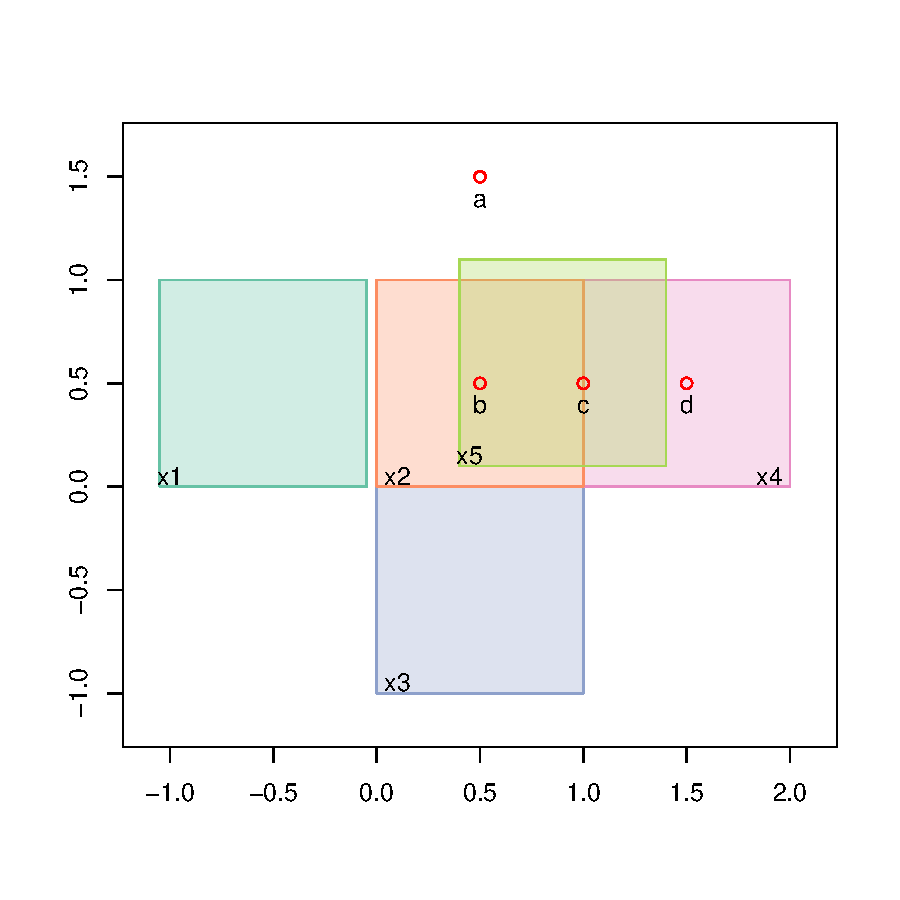
\includegraphics{over-005}
\caption{ Toy data: points (a-d), and (overlapping) polygons (x1-x5) }
\label{fig:toy}
\end{figure}

Now, the polygons \code{pol} in which points \code{pts} lie are
\begin{Schunk}
\begin{Sinput}
> over(pts, pol)
\end{Sinput}
\begin{Soutput}
 a  b  c  d 
NA  5  5  4 
\end{Soutput}
\end{Schunk}
As points \code{b} and \code{c} touch two overlapping polygons,
the output from the previous command does not provide all information
about the overlaps, only returning the \emph{last} polygon which touched
them (polygon 5 in both cases).
The complete information can be retrieved as a list:
\begin{Schunk}
\begin{Sinput}
> over(pts, pol, returnList = TRUE)
\end{Sinput}
\begin{Soutput}
$a
integer(0)

$b
[1] 2 5

$c
[1] 2 4 5

$d
[1] 4
\end{Soutput}
\end{Schunk}
This shows that \code{over} returns true if geometries in one element touch
geometries in another: they do not have to fully overlap
(see section \ref{dim} to constrain the selection criteria).
The points falling in or touching any of the polygons are selected by:
\begin{Schunk}
\begin{Sinput}
> pts[pol]
\end{Sinput}
\begin{Soutput}
SpatialPoints:
    x   y
b 0.5 0.5
c 1.0 0.5
d 1.5 0.5
Coordinate Reference System (CRS) arguments: NA 
\end{Soutput}
\end{Schunk}
The reverse, identical sequence of commands for 
selecting polygons \code{pol} that have 
(one or more) points of \code{pts} in them is done by
\begin{Schunk}
\begin{Sinput}
> over(pol, pts)
\end{Sinput}
\begin{Soutput}
x1 x2 x3 x4 x5 
NA  2 NA  3  2 
\end{Soutput}
\begin{Sinput}
> over(pol, pts, returnList = TRUE)
\end{Sinput}
\begin{Soutput}
$x1
integer(0)

$x2
[1] 2 3

$x3
integer(0)

$x4
[1] 3 4

$x5
[1] 2 3
\end{Soutput}
\begin{Sinput}
> row.names(pol[pts])
\end{Sinput}
\begin{Soutput}
[1] "x2" "x4" "x5"
\end{Soutput}
\end{Schunk}

\code{over} can also be used to query polygons in a single object overlay each other:

\begin{Schunk}
\begin{Sinput}
> if (require(rgeos, quietly = TRUE)) {
+  over(pol, pol, returnList = TRUE)
+ }
\end{Sinput}
\end{Schunk}

\noindent
The output tells us that \code{x1} does not intersect with any polygons other than itself, within the \code{pol} object. \code{x2} intersects with itself and \code{x3}, \code{x4} and \code{x5}, and so on.
Note that the \emph{types} of overlap queried by \code{over} include any intersecting points or edges under the \href{https://en.wikipedia.org/wiki/DE-9IM}{DE-9IM} standard.  More generic types of spatial overlap can be queried using functions from the rgeos package, as illustrated by the help page launched with \code{?rgeos::gRelate}.

Constraining polygon-polygon intersections to e.g. {\em overlap} using \code{over} is explained in section \ref{dim}.


\section{Using \code{over} to extract attributes}
\label{attr}

This section shows how \code{over(x,y)} is used to extract attribute
values of argument \code{y} at locations of \code{x}.  The return
value is either an (aggregated) data frame, or a list.

We now create an example \code{SpatialPointsDataFrame} and a
\code{SpatialPolygonsDataFrame} using the toy data created earlier:
\begin{Schunk}
\begin{Sinput}
> zdf = data.frame(z1 = 1:4, z2=4:1, f = c("a", "a", "b", "b"),
+ 	row.names = c("a", "b", "c", "d"))
> zdf
\end{Sinput}
\begin{Soutput}
  z1 z2 f
a  1  4 a
b  2  3 a
c  3  2 b
d  4  1 b
\end{Soutput}
\begin{Sinput}
> ptsdf = SpatialPointsDataFrame(pts, zdf)
> zpl = data.frame(z = c(10, 15, 25, 3, 0), zz=1:5, 
+ 	f = c("z", "q", "r", "z", "q"), row.names = c("x1", "x2", "x3", "x4", "x5"))
> zpl
\end{Sinput}
\begin{Soutput}
    z zz f
x1 10  1 z
x2 15  2 q
x3 25  3 r
x4  3  4 z
x5  0  5 q
\end{Soutput}
\begin{Sinput}
> poldf = SpatialPolygonsDataFrame(pol, zpl)
\end{Sinput}
\end{Schunk}

In the simplest example 
\begin{Schunk}
\begin{Sinput}
> over(pts, poldf)
\end{Sinput}
\begin{Soutput}
   z zz    f
a NA NA <NA>
b 15  2    q
c 15  2    q
d  3  4    z
\end{Soutput}
\end{Schunk}
a \code{data.frame} is created with each row corresponding to
the first element of the \code{poldf} attributes at locations
in \code{pts}.

As an alternative, we can pass a user-defined function to process
the table (selecting those columns to which the function makes sense):
\begin{Schunk}
\begin{Sinput}
> over(pts, poldf[1:2], fn = mean)
\end{Sinput}
\begin{Soutput}
    z       zz
a  NA       NA
b 7.5 3.500000
c 6.0 3.666667
d 3.0 4.000000
\end{Soutput}
\end{Schunk}

To obtain the complete list of table entries at each point of \code{pts}, 
we use the \code{returnList} argument:
\begin{Schunk}
\begin{Sinput}
> over(pts, poldf, returnList = TRUE)
\end{Sinput}
\begin{Soutput}
$a
[1] z  zz f 
<0 rows> (or 0-length row.names)

$b
    z zz f
x2 15  2 q
x5  0  5 q

$c
    z zz f
x2 15  2 q
x4  3  4 z
x5  0  5 q

$d
   z zz f
x4 3  4 z
\end{Soutput}
\end{Schunk}

The same actions can be done when the arguments are reversed:
\begin{Schunk}
\begin{Sinput}
> over(pol, ptsdf)
\end{Sinput}
\begin{Soutput}
   z1 z2    f
x1 NA NA <NA>
x2  2  3    a
x3 NA NA <NA>
x4  3  2    b
x5  2  3    a
\end{Soutput}
\begin{Sinput}
> over(pol, ptsdf[1:2], fn = mean)
\end{Sinput}
\begin{Soutput}
    z1  z2
x1  NA  NA
x2 2.5 2.5
x3  NA  NA
x4 3.5 1.5
x5 2.5 2.5
\end{Soutput}
\end{Schunk}

\section{Lines, and Polygon-Polygon overlays require {\tt rgeos}}

Package \code{sp} provides many of the \code{over} methods, but
not all.  Package \code{rgeos} can compute
geometry intersections, i.e. for any set of (points, lines,
polygons) to determine whether they have one ore more points in
common. This means that the \code{over} methods provided by package 
\code{sp}
can be completed by \code{rgeos} for {\em any} \code{over} methods
where a \code{SpatialLines} object is involved (either as \code{x}
or \code{y}), or where \code{x} and \code{y} are both of
class \code{SpatialPolygons} (table \ref{tab}). For this purpose,
objects of class \code{SpatialPixels} or \code{SpatialGrid} are
converted to \code{SpatialPolygons}. A toy example combines polygons
with lines, created by
\begin{Schunk}
\begin{Sinput}
> l1 = Lines(Line(coordinates(pts)), "L1")
> l2 = Lines(Line(rbind(c(1,1.5), c(1.5,1.5))), "L2")
> L = SpatialLines(list(l1,l2))
\end{Sinput}
\end{Schunk}
and shown in figure \ref{fig:lines}.

\begin{table}
\centering
\begin{tabular}{|l|ccccc|} \hline
              & y: Points & y: Lines & y: Polygons & y: Pixels & y: Grid \\
              \hline
x: Points        &   s    &    r     &      s      &      s    &  s  \\
x: Lines         &   r    &    r     &      r      &     r:y   & r:y \\
x: Polygons      &   s    &    r     &      r      &     s:y   & s:y \\
x: Pixels        &  s:x   &   r:x    &     s:x     &     s:x   & s:x \\ \hline
x: Grid          &  s:x   &   r:x    &     s:x     &     s:x   & s:x \\ \hline
\end{tabular}
\caption{ \code{over} methods implemented for different \code{x}
and \code{y} arguments.  s: provided by \pkg{sp}; r: provided by
\pkg{rgeos}. s:x or s:y indicates that the x or y argument is converted to grid
cell center points; r:x or r:y indicate grids or pixels are converted to
polygons equal to the grid cell. }
\label{tab}
\end{table}

\begin{figure}[htb]
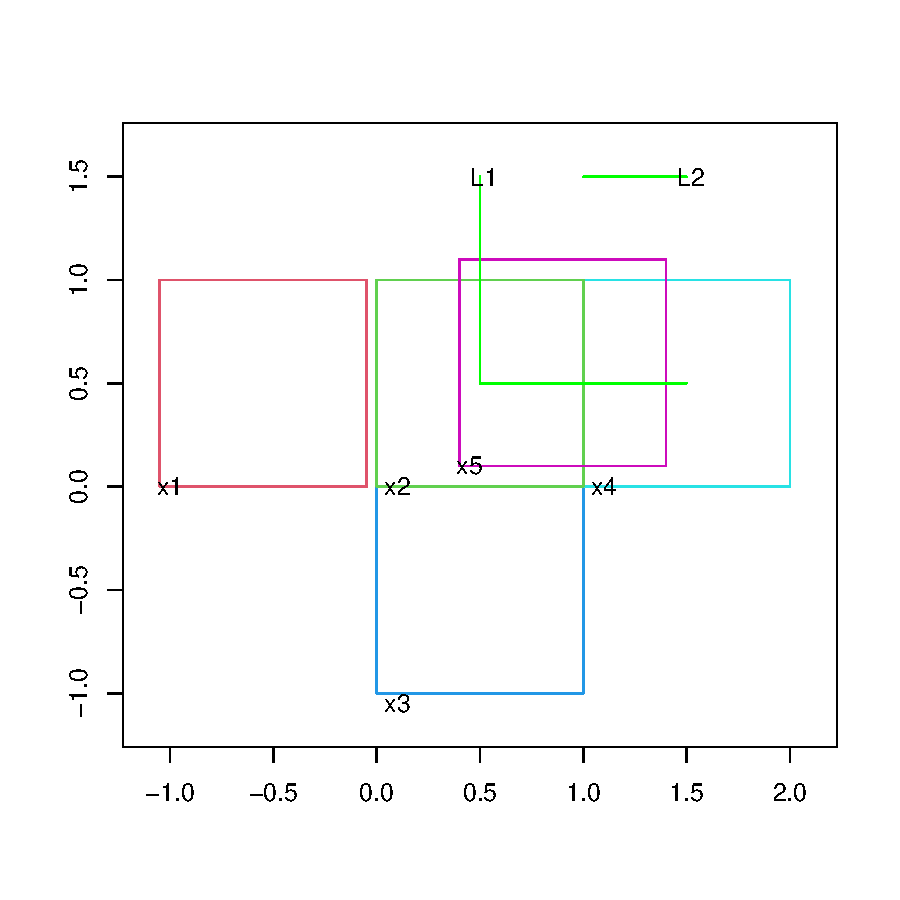
\includegraphics{over-017}
\caption{ Toy data: two lines and (overlapping) polygons (x1-x5) }
\label{fig:lines}
\end{figure}

The set of \code{over} operations on the polygons, lines and points 
is shown below (note that lists and vectors are named in this case):
\begin{Schunk}
\begin{Sinput}
> if (require(rgeos, quietly = TRUE)) {
+ over(pol, pol)
+ over(pol, pol,returnList = TRUE)
+ over(pol, L)
+ over(L, pol)
+ over(L, pol, returnList = TRUE)
+ over(L, L)
+ over(pts, L)
+ over(L, pts)
+ }
\end{Sinput}
\end{Schunk}

Another example overlays a line with a grid, shown in figure \ref{fig:grid}.
\begin{figure}
\begin{Schunk}
\begin{Sinput}
> data(meuse.grid)
> gridded(meuse.grid) = ~x+y
> Pt = list(x = c(178274.9,181639.6), y = c(329760.4,333343.7))
> sl = SpatialLines(list(Lines(Line(cbind(Pt$x,Pt$y)), "L1")))
> image(meuse.grid)
> if (require(rgeos, quietly = TRUE)) {
+  xo = over(sl, geometry(meuse.grid), returnList = TRUE)
+  image(meuse.grid[xo[[1]], ],col=grey(0.5),add=T)
+  lines(sl)
+ }
\end{Sinput}
\end{Schunk}
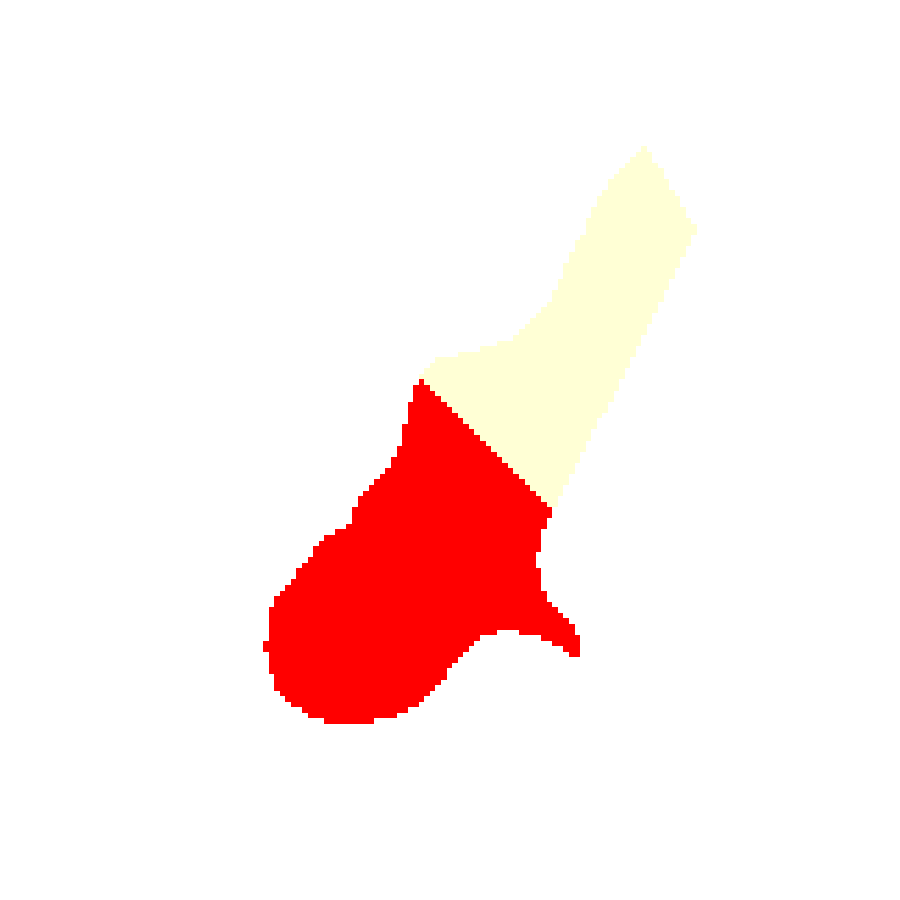
\includegraphics{over-019}
\caption{ Overlay of line with grid, identifying cells crossed (or touched)
by the line }
\label{fig:grid}
\end{figure}

\section{Ordering and constraining of \code{rgeos}-based intersects}

Consider the following ``identical'' $3 \times 3$ grid, represented as 
\code{SpatialGrid}, \code{SpatialPolygons} and \code{SpatialPixels}:
\begin{Schunk}
\begin{Sinput}
> g = SpatialGrid(GridTopology(c(0,0), c(1,1), c(3,3)))
> p = as(g, "SpatialPolygons")
> px = as(g, "SpatialPixels")
> plot(g)
> text(coordinates(g), labels = 1:9)
\end{Sinput}
\end{Schunk}
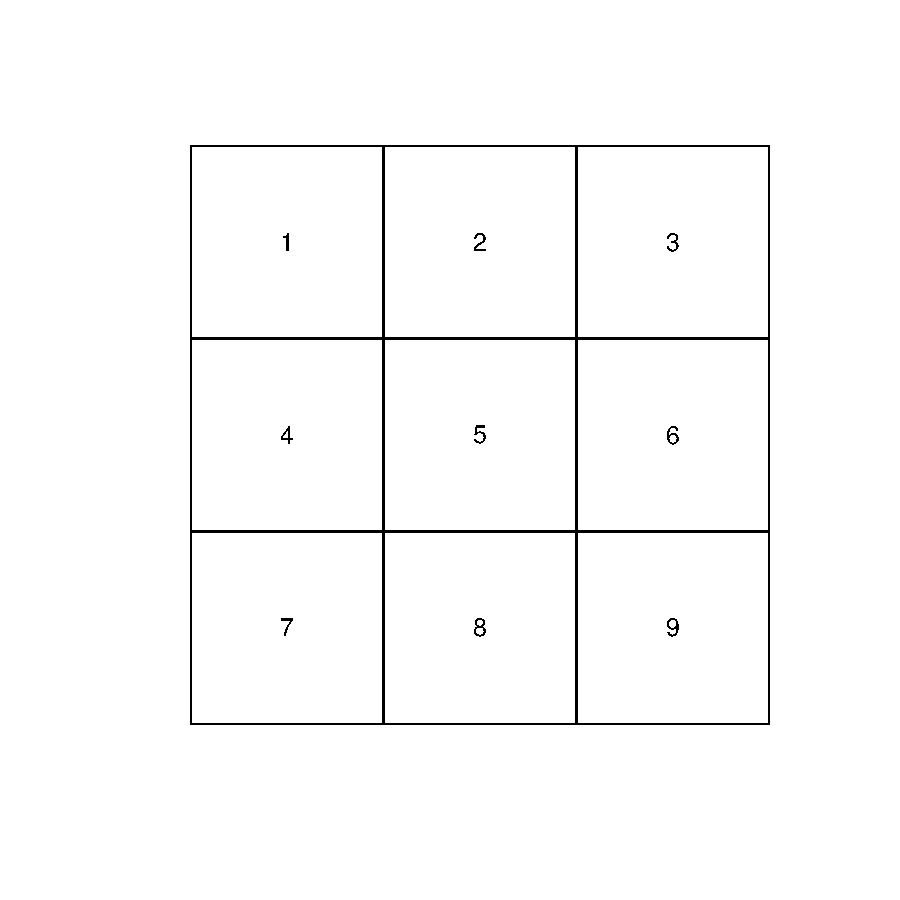
\includegraphics{over-020}

We can match these geometries with themselves by
\begin{Schunk}
\begin{Sinput}
> if (require(rgeos, quietly = TRUE)) {
+ over(g,g)
+ over(p,p)
+ over(p,g)
+ over(g,p)
+ }
\end{Sinput}
\end{Schunk}
and see that most give a 1:1 match, except for polygons-polygons \code{(p,p)}.

When we ask for the full set of matches, we see
\begin{Schunk}
\begin{Sinput}
> if (require(rgeos, quietly = TRUE)) {
+ over(px[5], g, returnList = TRUE)
+ over(p[c(1,5)], p, returnList = TRUE)
+ }
\end{Sinput}
\end{Schunk}
and note that the implementation lets grids/pixels not match
(intersect) with neighbour grid cells, but that polygons do. 

There are two issues we'd like to improve here: the order in
which matching features (here: polygons) are returned, and the
possibility to limit this by the dimension of the intersection
(point/line/area). Both will be explained now.

\subsection{Ordering of matches}

By default, polygon-polygon features are matched by
\code{rgeos::gIntersects}, which just returns {\em any} match in
{\em any} order (feature order, it seems). Although it is slower,
we  can however improve on this by switching to \code{rgeos::gRelate}, and see
\begin{Schunk}
\begin{Sinput}
> if (require(rgeos, quietly = TRUE)) {
+ over(px[5], g, returnList = TRUE, minDimension = 0)
+ over(p[c(1,5)], p, returnList = TRUE, minDimension = 0)
+ }
\end{Sinput}
\end{Schunk}
When \code{minDimension = 0} is specified, the matching geometries
are being returned based on a nested ordering. First, ordering
is done by dimensionality of the intersection, as returned
by the \code{rgeos} function \code{gRelate} (which uses the
\href{https://en.wikipedia.org/wiki/DE-9IM}{DE-9IM} model).
This means that features that have an area overlapping (dim=2)
are listed before features that have a line in common (dim=1),
and that line in common features are listed before features that
only have a point in common (dim=0).

Remaining ties, indicating cases when there are multiple different
intersections of the same dimension, are ordered such that matched
feature {\em interiors} are given higher priority than matched
feature boundaries.

Note that the ordering also determines which feature is matched
when \code{returnList=FALSE}, as in this case the first element of
the ordered set is taken:
\begin{Schunk}
\begin{Sinput}
> if (require(rgeos, quietly = TRUE)) {
+ over(p, p, minDimension = 0)
+ }
\end{Sinput}
\end{Schunk}

Consider the following example where a point is {\em on} \code{x1} and {\em in} \code{x2}: 
\begin{Schunk}
\begin{Sinput}
> x2 = x1 = cbind(c(0,1,1,0,0), c(0,0,1,1,0))
> x1[,1] = x1[,1]+0.5
> x1[,2] = x1[,2]+0.25
> sp = SpatialPolygons(list(
+  Polygons(list(Polygon(x1)), "x1"),
+  Polygons(list(Polygon(x2)), "x2")))
> pt = SpatialPoints(cbind(0.5,0.5)) # on border of x1
> row.names(pt) = "pt1"
> plot(sp, axes = TRUE)
> text(c(0.05, 0.55, 0.55), c(0.9, 1.15, 0.5), c("x1","x2", "pt"))
> plot(pt, add=TRUE, col='red', pch=16)
\end{Sinput}
\end{Schunk}
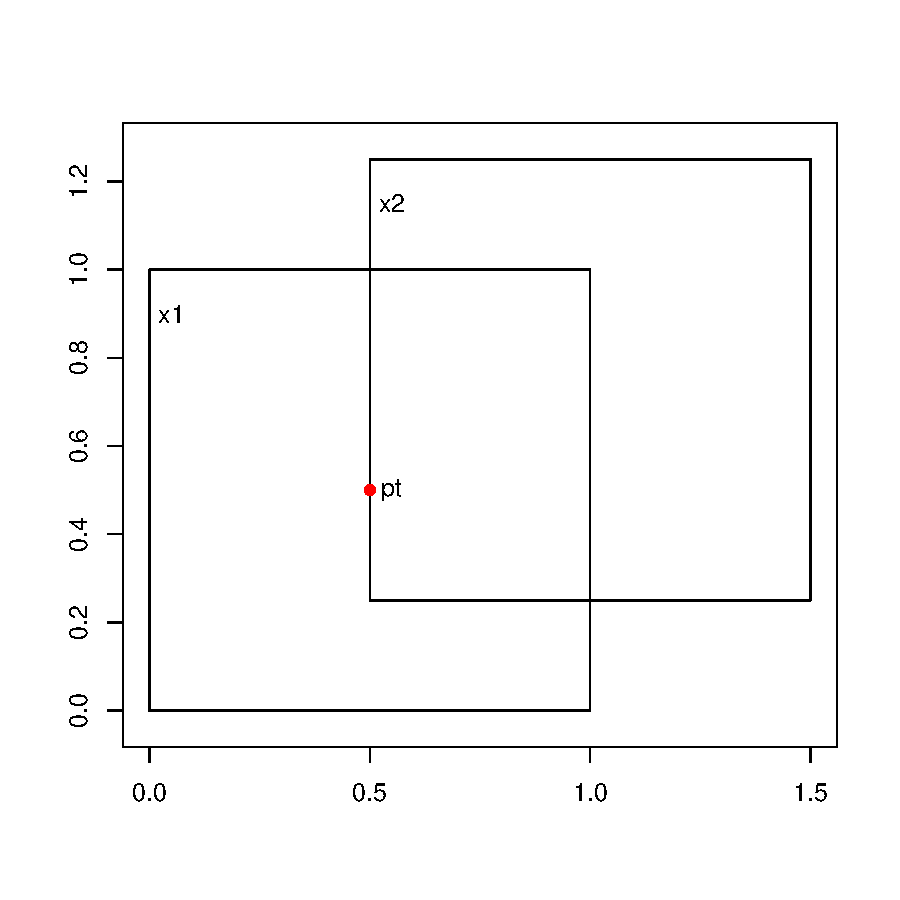
\includegraphics{over-025}

When matching the point \code{pt} with the two polygons, the
sp method (default) gives no preference of the second polygon
that (fully) contains the point; the rgeos method however does:
\begin{Schunk}
\begin{Sinput}
> if (require(rgeos, quietly = TRUE)) {
+ over(pt,sp)
+ over(pt,sp,minDimension=0)
+ over(pt,sp,returnList=TRUE)
+ rgeos::overGeomGeom(pt,sp)
+ rgeos::overGeomGeom(pt,sp,returnList=TRUE)
+ rgeos::overGeomGeom(pt,sp,returnList=TRUE,minDimension=0)
+ }
\end{Sinput}
\end{Schunk}

% #    x1     x2 
% #	"F0FF" "0FFF" 
% # it would be nice to have these sorted "2, 1" instead of "1, 2", but
% # that doesn't work now.

\subsection{Constraining dimensionality of intersection}
\label{dim}

In some cases for feature selection it may be desired to constrain
matching to features that have an area overlap, or that have an
area overlap {\em or} line in common. This can be done using the
parameter \code{minDimension}:

\begin{Schunk}
\begin{Sinput}
> if (require(rgeos, quietly = TRUE)) {
+ over(p[5], p, returnList=TRUE, minDimension=0)
+ over(p[5], p, returnList=TRUE, minDimension=1)
+ over(p[5], p, returnList=TRUE, minDimension=2)
+ rgeos::overGeomGeom(pt, pt, minDimension=2) # empty
+ rgeos::overGeomGeom(pt, pt, minDimension=1) # empty
+ rgeos::overGeomGeom(pt, pt, minDimension=0)
+ }
\end{Sinput}
\end{Schunk}

\section{Aggregation}
In the following example, the values of a fine grid with 40 m x 40
m cells are aggregated to a course grid with 400 m x 400 m cells.
\begin{Schunk}
\begin{Sinput}
> data(meuse.grid)
> gridded(meuse.grid) = ~x+y
> off = gridparameters(meuse.grid)$cellcentre.offset + 20
> gt = GridTopology(off, c(400,400), c(8,11))
> SG = SpatialGrid(gt)
> agg = aggregate(meuse.grid[3], SG, mean)
\end{Sinput}
\end{Schunk}
Figure \ref{fig:agg} shows the result of this aggregation
(\code{agg}, in colors) and the points (+) of the original grid
(\code{meuse.grid}). Function \code{aggregate} aggregates its first
argument over the geometries of the second argument, and returns
a geometry with attributes.  The default aggregation function
(\code{mean}) can be overridden.

\begin{figure}[htb]
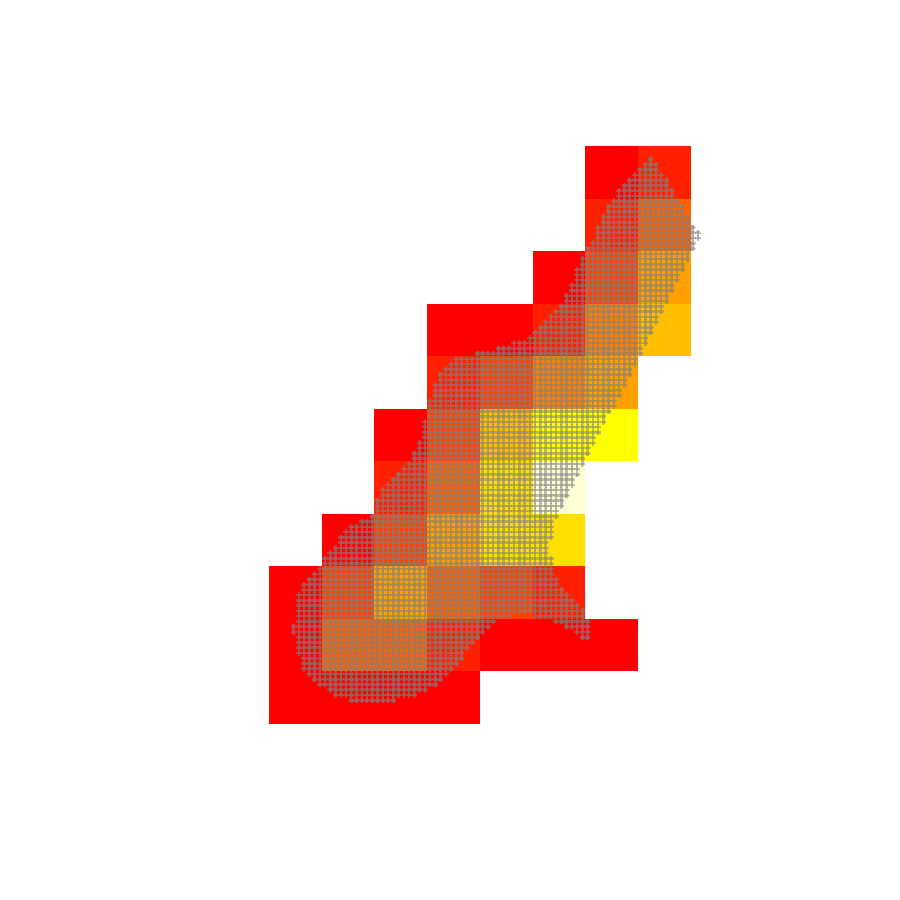
\includegraphics{over-029}
\caption{ aggregation over meuse.grid distance values to a 400 m
x 400 m grid}
\label{fig:agg}
\end{figure}

An example of the aggregated values of \code{meuse.grid} along
(or under) the line shown in Figure \ref{fig:lines} are
\begin{Schunk}
\begin{Sinput}
> if (require(rgeos, quietly = TRUE)) {
+ sl.agg = aggregate(meuse.grid[,1:3], sl, mean)
+ class(sl.agg)
+ as.data.frame(sl.agg)
+ }
\end{Sinput}
\end{Schunk}
Function \code{aggregate} returns a spatial object of the same
class of \code{sl} (\code{SpatialLines}), and \code{as.data.frame}
shows the attribute table as a \code{data.frame}.

\subsection{Constraining the dimension of intersection}
Building on the simple example of section \ref{dim}, 
we can see what happens if we aggregate polygons {\em without}
specifying {\em how} polygons intersect\footnote{sp versions
1.2-1, rgeos versions 0.3-13}, the result of which is shown
in Figure \ref{fig:agg}.

\begin{Schunk}
\begin{Sinput}
> if (require(rgeos, quietly = TRUE)) {
+ g = SpatialGrid(GridTopology(c(5,5), c(10,10), c(3,3)))
+ p = as(g, "SpatialPolygons")
+ p$z = c(1,0,1,0,1,0,1,0,1)
+ cc = coordinates(g)
+ p$ag1 = aggregate(p, p, mean)[[1]]
+ p$ag1a = aggregate(p, p, mean, minDimension = 0)[[1]]
+ p$ag2 = aggregate(p, p, mean, minDimension = 1)[[1]]
+ p$ag3 = aggregate(p, p, mean, minDimension = 2)[[1]]
+ p$ag4 = aggregate(p, p, areaWeighted=TRUE)[[1]]
+ }
\end{Sinput}
\end{Schunk}

\begin{figure}[ht]
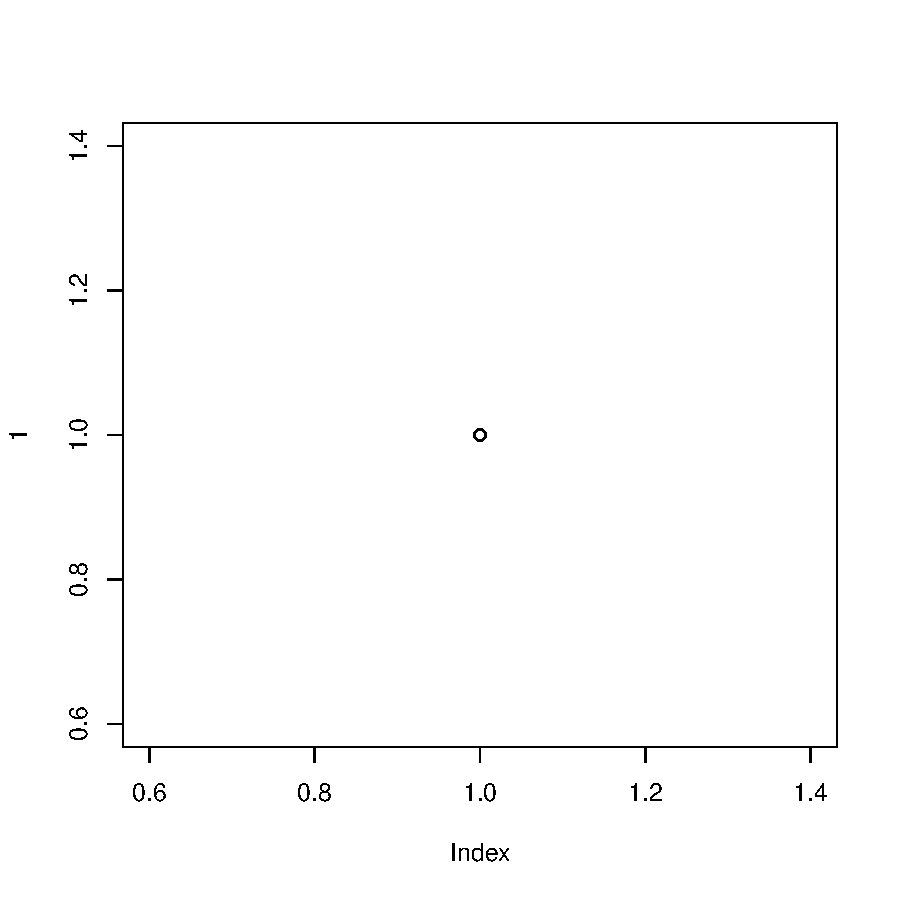
\includegraphics{over-032}
\caption{Effect of aggregating checker board {\tt SpatialPolygons} by themselves, for
different values of {\tt minDimension} and {\tt areaWeighted}; the green square example
is given in the text.}
\label{fig:agg}
\end{figure}

The option \code{areaWeighted=TRUE} aggregates area-weighted,
giving zero weight to polygons that only have a point or line in
common with the target polygon; \code{minDimension} is passed to
\code{over} to constrain the intersecting polygons used.

The following example furher illustrates the difference between selection
using {\tt minDimension}, and area weighting for aggregating the 0-1 checker
board of figure \ref{fig:agg} by the green square polygon ({\tt sq}) 
shown in the last panel of that figure:
\begin{Schunk}
\begin{Sinput}
> if (require(rgeos, quietly = TRUE)) {
+ round(c(
+   aggDefault = aggregate(p, sq, mean)[[1]],
+   aggMinDim0 = aggregate(p, sq, mean, minDimension = 0)[[1]],
+   aggMinDim1 = aggregate(p, sq, mean, minDimension = 1)[[1]],
+   aggMinDim2 = aggregate(p, sq, mean, minDimension = 2)[[1]],
+   areaWeighted = aggregate(p, sq, areaWeighted=TRUE)[[1]]), 3)
+ }
\end{Sinput}
\end{Schunk}



\section*{References}
\begin{itemize}
\item O'Sullivan, D., Unwin, D. (2003) Geographical Information
Analysis. Wiley, NJ.
\item
Davidson, R., 2008.  Reading topographic maps. Free e-book from:
\url{http://www.map-reading.com/}
\item
Heuvelink, G.B.M., and E.J. Pebesma, 1999.  Spatial aggregation
and soil process modelling. Geoderma 89, 1-2, 
\href{http://dx.doi.org/10.1016/S0016-7061(98)00077-9}{47-65}.
\item
Pebesma, E., 2012.  Spatio-temporal overlay and
aggregation.  Package vignette for package spacetime,
\url{https://cran.r-project.org/web/packages/spacetime/vignettes/sto.pdf}

\end{itemize}

\end{document}
